\section{Problem No.2}
\subsection{Problem Description:} 
Consider the following PDE:
$$u_{t} = 0.01u_{xx}+1-exp(-t),\;\; 0<x<1$$
$$u(0,t) =0,\;\; u(1,t)=0$$
$$u(x,0)=0 $$
Write a program to solve the problem using Crank-Nicolson up to time $t=1$, and perform a refinement study that demonstrates that the method is second-order accurate in space and time. 

\subsection{Solution:} \label{prob2_sol}

The discretized PDE under Crank-Nicolson scheme is\cite{hoffmann2000computational}:

$$
\frac{u_{i}^{n+1}-u_{i}^{n}}{\Delta t} = \frac{1}{2} (0.01(\frac{u_{i+1}^{n+1} -2u_{i}^{n+1}+u_{i-1}^{n+1}}{(\Delta x)^{2}}+\frac{u_{i+1}^{n} -2u_{i}^{n}+u_{i-1}^{n}}{(\Delta x)^{2}}) - exp(-n\Delta t)(1+exp(\Delta t)))
$$
where $\Delta t$ is the time spacing and $\Delta x$ is the space spacing. The left side is central difference with time-step $\frac{ \Delta t}{2}$, and the right side is the average of two central difference second order derivative. Thus the scheme is second-order accurate in space and time. 

The equation can be rearranged as follows
$$
(1+\Delta t\frac{0.01}{(\Delta x)^{2}})u_{i}^{n+1} - \frac{\Delta t}{2}\frac{0.01}{(\Delta x)^{2}}u_{i+1}^{n+1}-\frac{\Delta t}{2}\frac{0.01}{(\Delta x)^{2}}u_{i-1}^{n+1} =
\\
\qquad (1-\Delta t \frac{0.01}{(\Delta x)^{2}})u_{i}^{n} + \frac{\Delta t}{2}\frac{0.01}{(\Delta x)^{2}}(u_{i+1}^{n} +u_{i-1}^{n}) - \frac{\Delta t}{2}(2-exp(-n\Delta t)-exp(-(n+1)\Delta t))
$$
or
$$
Au_{i}^{n+1} + Bu_{i+1}^{n+1} +Cu_{i-1}^{n+1} = D_{i}^{n}
$$
\vspace{0.2mm}

where $A = (1+\Delta t \frac{0.01}{(\Delta x)^{2}}), \; B=C=- \frac{\Delta t}{2}\frac{0.01}{(\Delta x)^{2}}$ and $$D_{i}^{n}=(1-\Delta t \frac{0.01}{(\Delta x)^{2}})u_{i}^{n} + \frac{\Delta t}{2}\frac{0.01}{(\Delta x)^{2}}(u_{i+1}^{n} +u_{i-1}^{n}) - \frac{\Delta t}{2}(2-exp(-n\Delta t)-exp(-(n+1)\Delta t))$$

Knowing the boundary and initial condition, the formula can be used to solve the internal gird points i.e., $0<i<nx-1$, and $0<n<ny$ where $nx$ is the number of grid points in the space direction and $ny$ is the number of gird points in time direction. 

\vspace{2mm}

For $i=1\longrightarrow Au_{1}^{n+1} +Bu_{2}^{n+1} +Cu_{0}^{n+1} = D_{1}^{n}$

\vspace{2mm}

or $Au_{1}^{n+1} +Bu_{2}^{n+1} = D_{1}^{n} -Cu_{0}^{n+1}$

\vspace{2mm}

For $i=2\longrightarrow Au_{2}^{n+1} +Bu_{3}^{n+1} +Cu_{1}^{n+1} = D_{2}^{n}$

\vspace{2mm}

For $i=3\longrightarrow Au_{3}^{n+1} +Bu_{4}^{n+1} +Cu_{2}^{n+1} = D_{3}^{n}$

And so forth, till we reach $i=nx-2$

\vspace{2mm}

For $i=nx-2\longrightarrow Au_{nx-2}^{n+1} +Bu_{nx-1}^{n+1} +Cu_{nx-3}^{n+1} = D_{nx-2}^{n}$

\vspace{2mm}

or $ Au_{nx-2}^{n+1} +Cu_{nx-3}^{n+1} = D_{nx-2}^{n} - Bu_{nx-1}^{n+1}$

\vspace{2mm}

This will give a system of equation that can be represented by a tri-diagonal matrix as follows 


\[
\left| \begin{array}{ccc ccccc}
A & B & 0 & 0 & ... & ... & 0 & 0 \\
C & A & B & 0 & ... & ... & 0 & 0 \\
0 & C & A & B & ... & ... & 0 & 0\\
... & ... & ... & ... & ... & ... & ... & ...\\
... & ... & ... & ... & ... & ... & ... & ...\\
... & ... & ... & ... & ... & ... & ... & ...\\
0 & 0 & ... & ... & 0 & C & A & B\\
0 & 0 & ... & ... & 0 & 0 & C & A\\
\end{array} \right|
\left| \begin{array}{c}
u_{1}^{n+1} \\
u_{2}^{n+1} \\
u_{3}^{n+1} \\
...\\
...\\
...\\
u_{nx-3}^{n+1}\\
u_{nx-2}^{n+1}\\
\end{array} \right|
=
\left| \begin{array}{c}
D_{1}^{n}-Cu_{0}^{n+1} \\
D_{2}^{n} \\
D_{3}^{n} \\
...\\
...\\
...\\
D_{nx-3}^{n} \\
D_{nx-2}^{n}-Bu_{nx-1}^{n+1} \\
\end{array} \right|
\] 

The system is then solved using LU-Decomposition. 
 
\subsection{Results:}
Using the above formula, we can obtain the solution for different grid resolution as shown in Figure \ref{fig:CN2}. For each grid resolution, we calculated the solution at different time steps (x-axis) and plotted them against the space (y-axis). For the iso-contour, red color means the function value is close to 1 while blue is for function values closer to 0. We notice that at different grid resolution, the effect of the boundary wash out as we advance in time. Additionally, the rate of washing out (convergence) is accelerated by increasing the grid resolution. 

\begin{figure}[tbh]
 \centering  
   {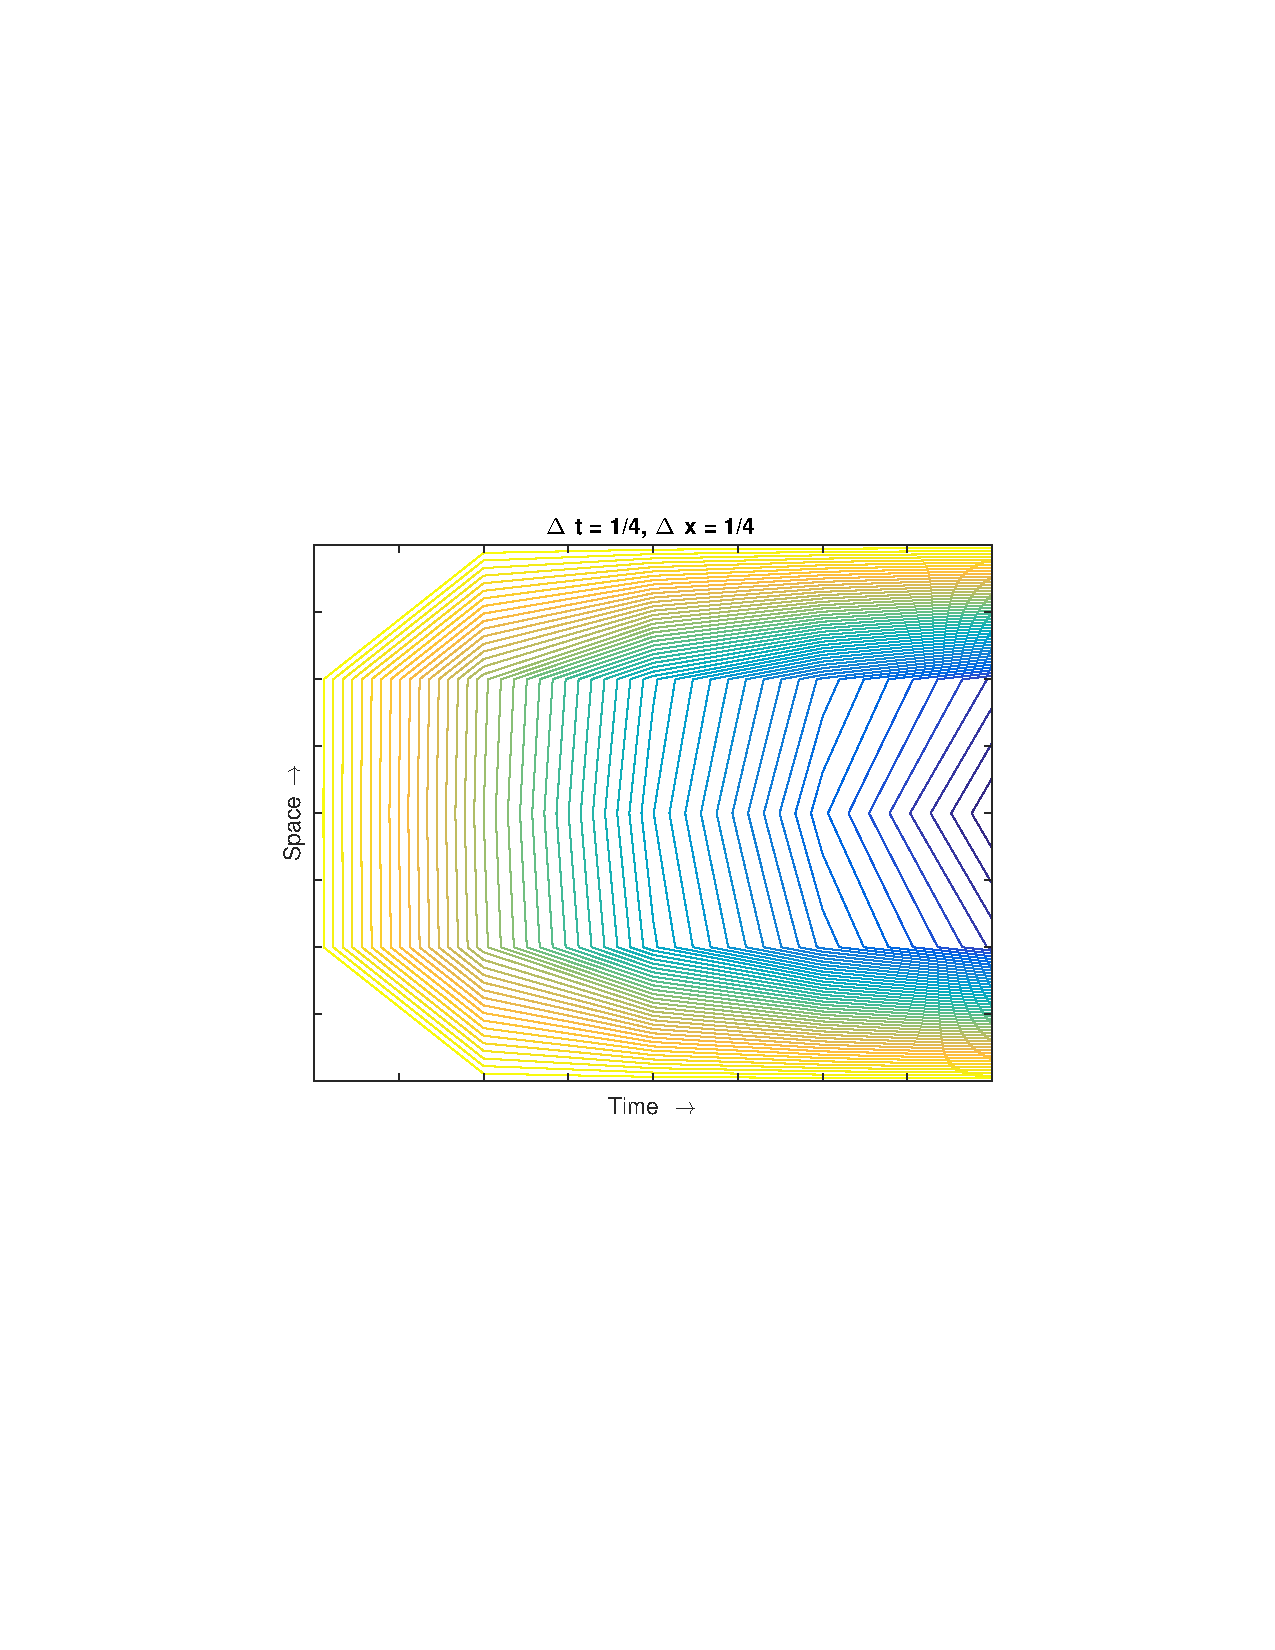
\includegraphics[width=0.3\linewidth]{fig/X4_T4.pdf}}
   \quad
   {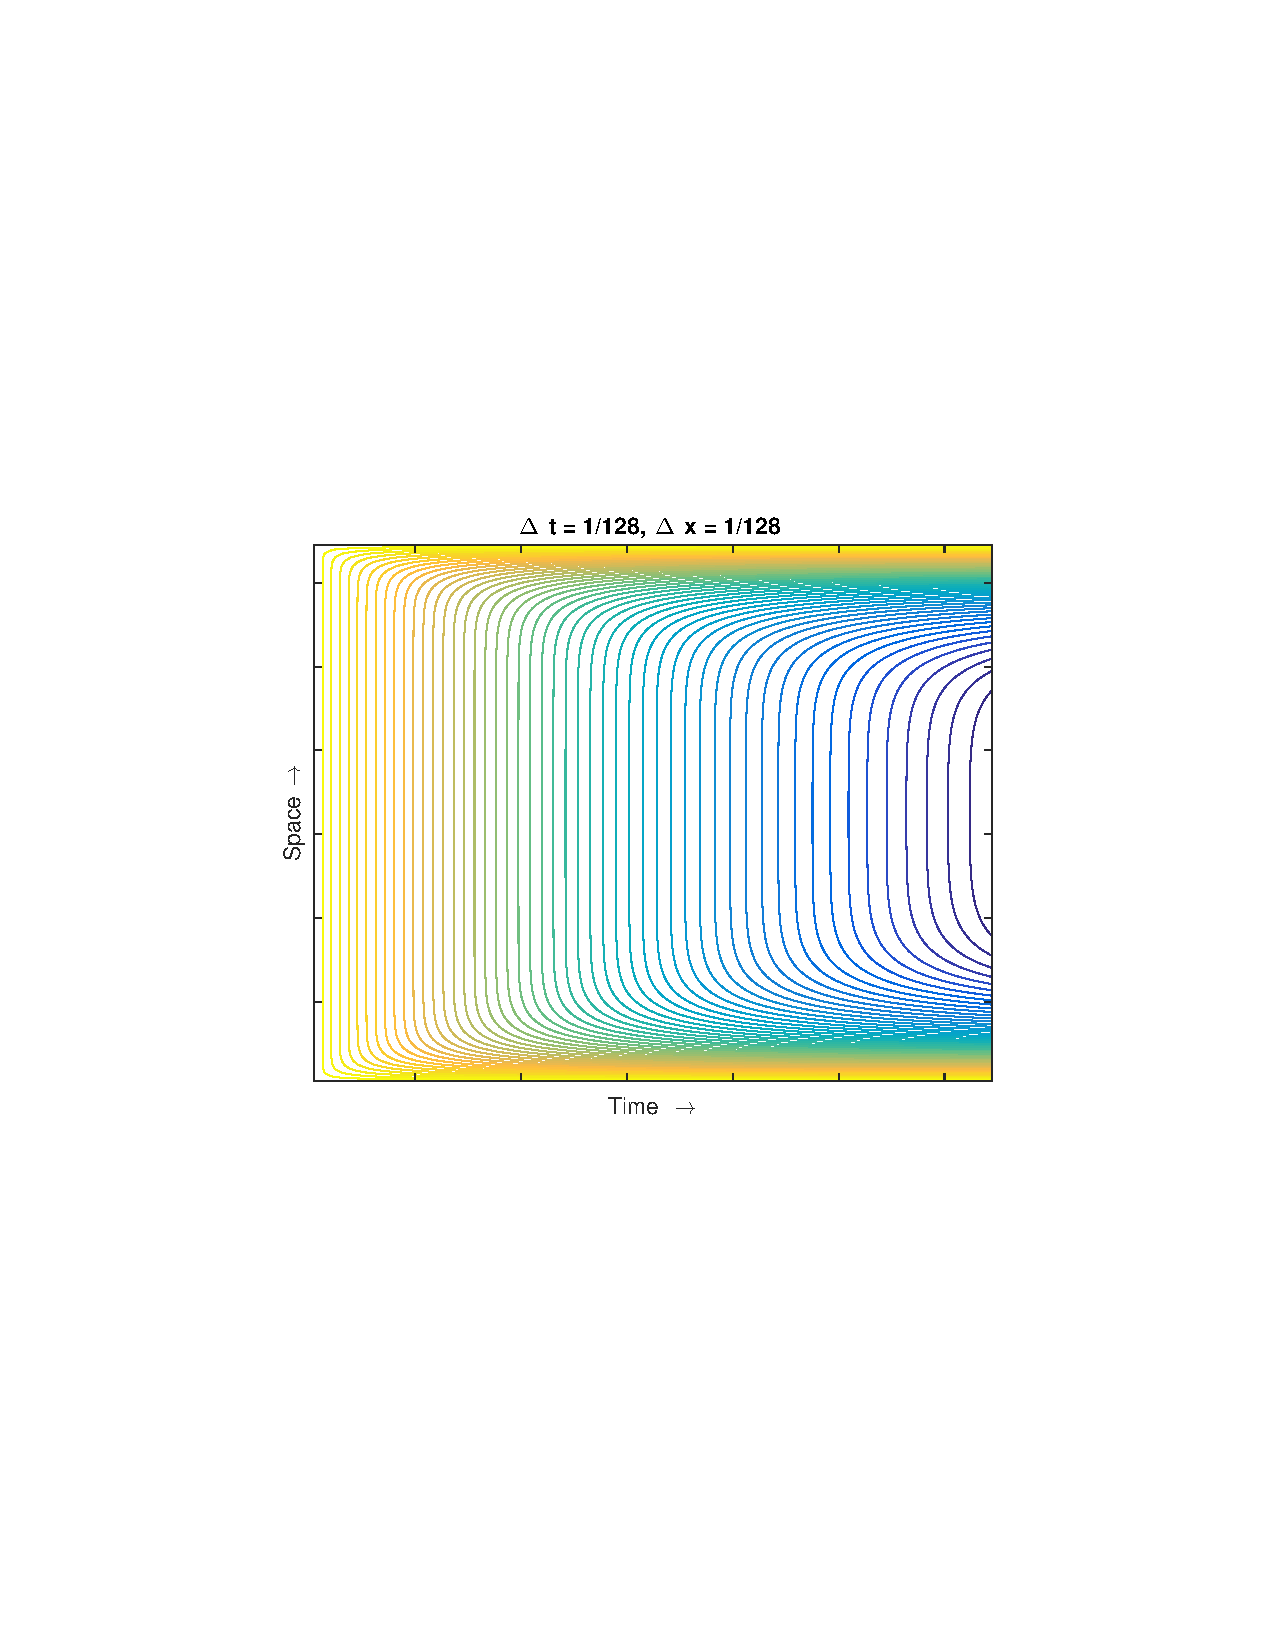
\includegraphics[width=0.3\linewidth]{fig/X128_T128.pdf}}
   \quad
   {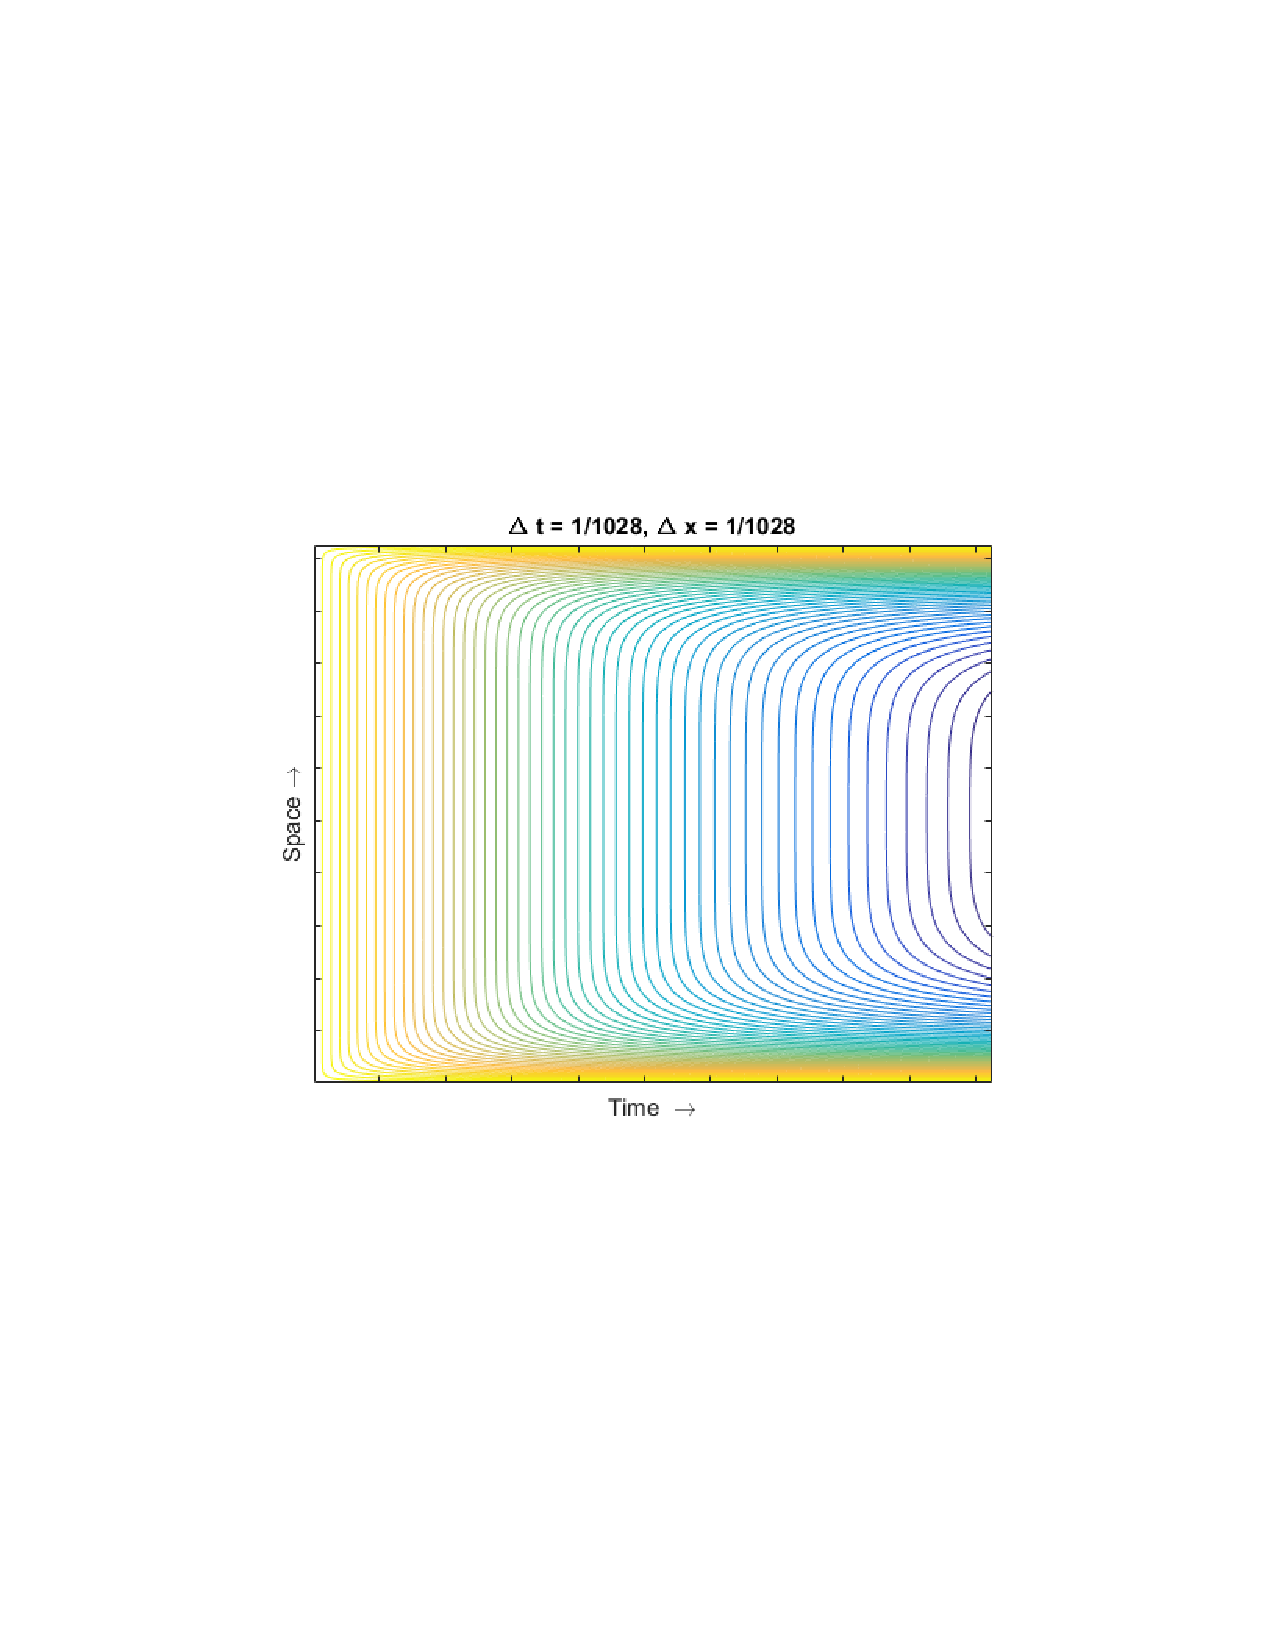
\includegraphics[width=0.3\linewidth]{fig/X1024_T1024.pdf}}
  \caption{Iso-contour of the the solution for the given PDE using Crank-Nicolson scheme for different $\Delta t$ and $\Delta x$ values. The horizontal axis represents the time (advances from right to left) while the vertical axis represents the space.}
   \label{fig:CN2}
\end{figure} 

\paragraph{Refinement Study:} The goal of this study is to confirm that Crank-Nicolson scheme is second-order accurate in space and time. Ideally, we would calculate the solution for different grid resolution and graph the error as the normalized difference from the analytical solution. Since the analytical solution is not provided, and since we are interested only in the order of the error, we can calculate it based on the relative error between each two successive grid resolution. 

\subparagraph{Methodology:} Here we derive how to extract the order of accuracy without the analytical solution. We are going to derive the order of $n$ order forward finite different equation $f^{\prime}(x_{o}) = \frac{f(x_{o}+ih_{1})}{h_{1}} + (O(h_{1}))^{n}$ where $h_{1}$ is the grid spacing. We can write the same equation for the same $x_{o}$ for another grid resolution $h_{2}$ and subtract. The result would be
$$
\frac{f(x_{o}+ih_{1})}{h_{1}} - \frac{f(x_{o}+ih_{2})}{h_{2}} = (O(h_{2}))^{n}-(O(h_{1}))^{n}
$$
The LHS represents the difference between two solution computed for two different grid resolution. Thus, we can substitute it symbolically by $C_{1} - C_{2} = (O(h_{2}))^{n}-(O(h_{1}))^{n}$;
where $C_{1}$ and $C_{2}$ represent the computed solution. Additionally, we can represent the RHS by a single term of order $n$ since we are looking for the order not the exact value. This simplifies the equation to be 
$C_{1} - C_{2} = (Error)^{n}$, where $Error$ is a function of grid spacing. By taking the log of both sides, the equations becomes $log(C_{1} - C_{2}) = n*log(Error)$. Thus, by taking the difference of two successive solutions at a point in time, and draw this difference against the grid spacing on log-log scale, the results is a straight line whose slope is the order of accuracy. So, we computed the solution at time =1 for certain refinement level and then compute the normalized sum. We did the same thing for another refinement level. The difference between the two normalized sums substitutes $C_{1}-C_{2}$ in the above equation. Note that this is the error over both space and time. 

We use the same method with different space and time steps. We starts by 4 space and time steps and increase both by factor of 2 at each solution. We plot the total difference between each two successive solution at $t=1$ against the grid resolution on a log-log scale (Figure \ref{fig:ref}). We notice that the first point does not lie on the same line. This point is computed as the error between grid of size $4\times4$ and $8\times8$ which is too coarse and the results generally could be considered unreliable. The slope of the resulting line is -2.1. Thus, we can conclude that the method is second order accurate in space and time. 
 
 \begin{figure}[!tbh]
 \centering  
   {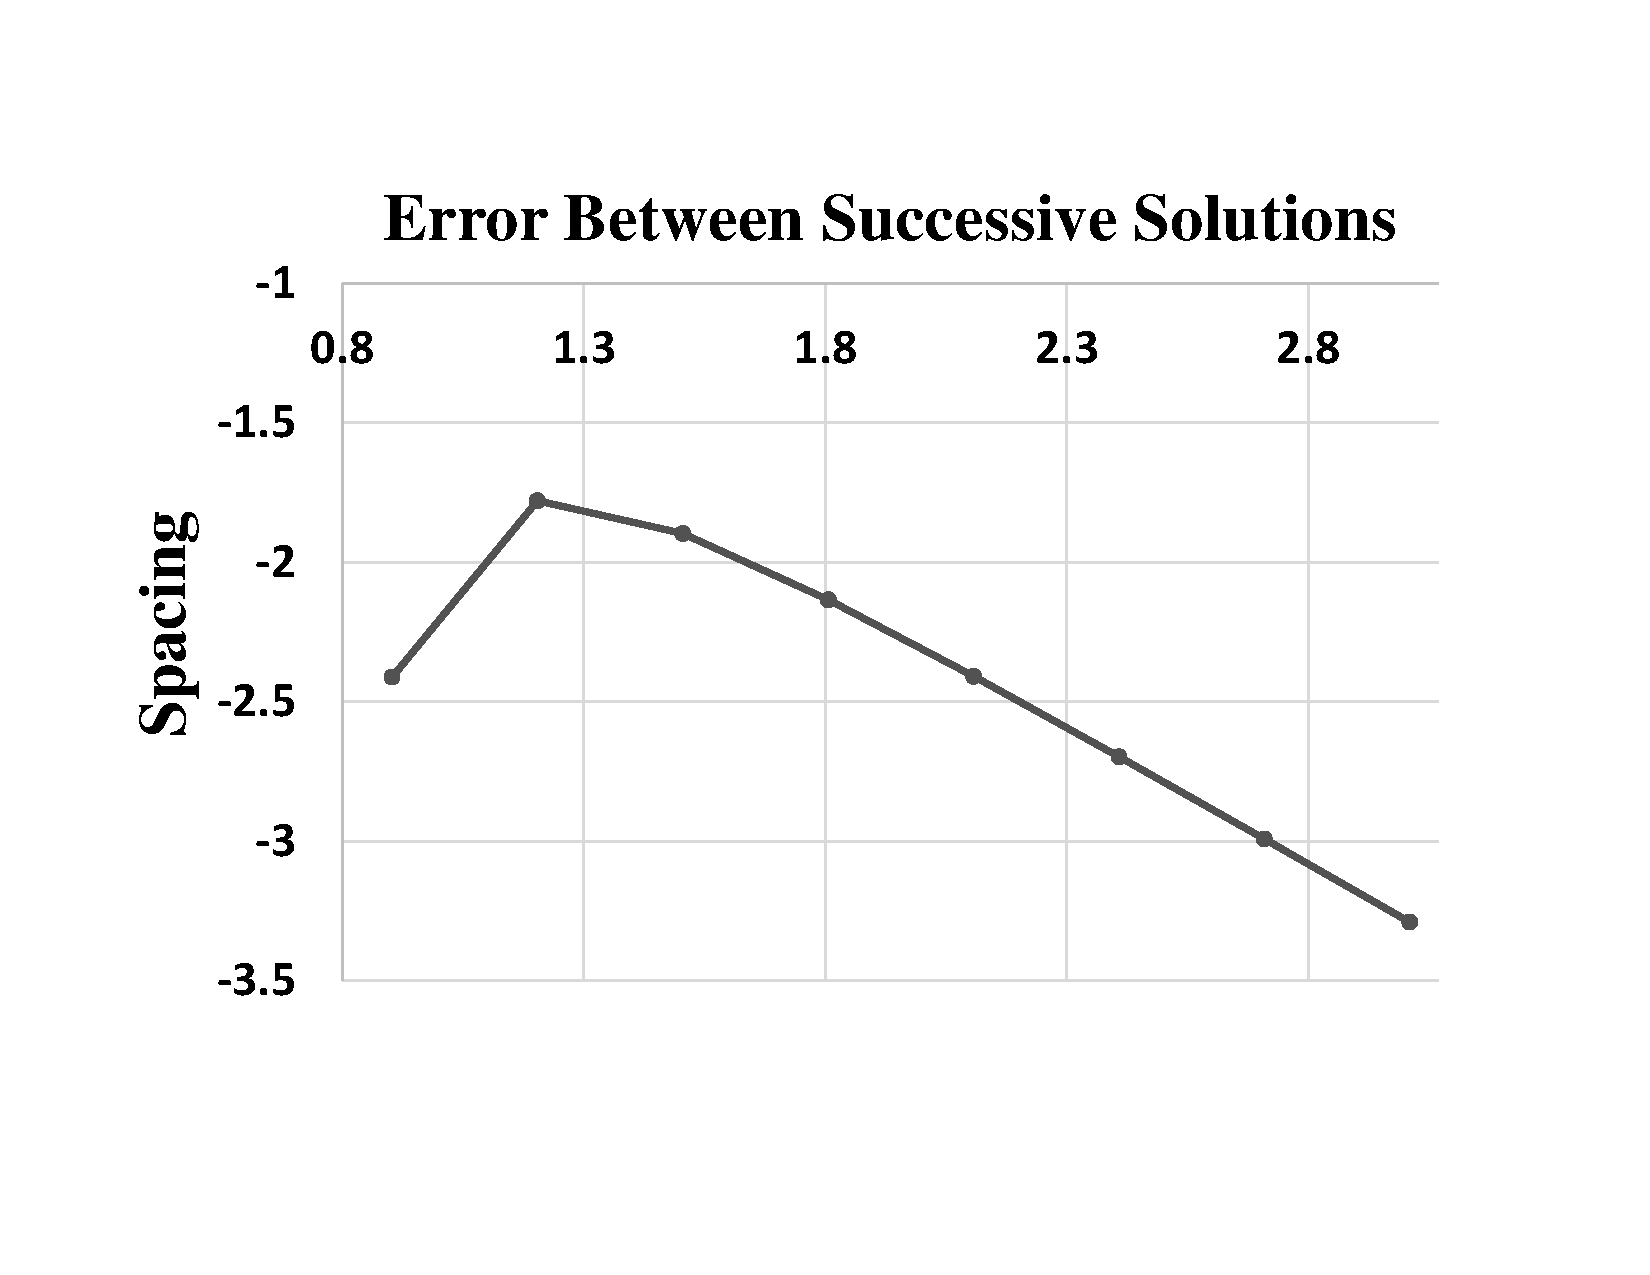
\includegraphics[width=0.6\linewidth]{fig/ref_study_prob2.pdf}}   
  \caption{For the refinement study, we draw the error between two successive solution at $t=1$ for different grid resolution and the slope of output line represents the order of accuracy in space and time.}
   \label{fig:ref}
\end{figure} 